% made with PGFPlotsEdt
\documentclass[tikz]{standalone}
\usepackage{pgfplots}
\pgfplotsset{compat=newest}
\usepgfplotslibrary{colorbrewer}
\usepgfplotslibrary{colormaps}
\begin{document}
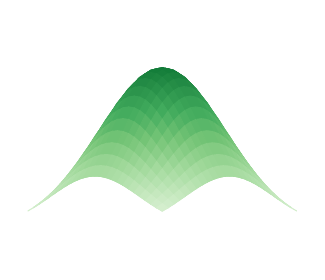
\begin{tikzpicture}
\begin{axis}[width={5cm},
height={5cm},
axis x line={none},
axis y line={none},
view={45}{0},
axis z line={none},
colormap/Greens]
 \addplot3 [domain=0:2*pi,color=green!25!black!50!white,mesh,line width=1.8pt,samples=100,samples y=0,opacity=0] ({1.18*cos(deg(x))},{1.18*cos(deg(x))},{0.7*sin(deg(x))-0.15});
 \addplot3 [domain=-1.5:1.5,surf,shader=flat] {exp(-x^2/2-y^2/2)-0.7};
\end{axis}
\end{tikzpicture}
\end{document}